%!TEX program = lualatex
\documentclass[ngerman,headheight=70pt]{scrartcl}
\usepackage[ngerman]{babel}
\usepackage{blindtext}
\usepackage[utf8]{luainputenc}
\usepackage{scrlayer-scrpage}
\usepackage[T1]{fontenc}
\usepackage{fontspec}
\usepackage{multicol}
\usepackage{enumitem}
\usepackage[german=quotes]{csquotes}
\usepackage[bottom=2cm,footskip=8mm]{geometry}
\usepackage{pdfpages}
\setmainfont{Source Sans Pro}
\MakeOuterQuote{"}

\setlength{\parindent}{0pt}
\setlength{\parskip}{6pt}

\pagestyle{plain.scrheadings}
\thispagestyle{scrheadings}
\lohead{\vspace*{-1.5cm}
\includegraphics[scale=0.4]{../images/stupa_logo_rot.pdf}}
\rohead{\\Präsidium des\\Studierendenparlaments}

\lofoot[Universität Hamburg · Präsidium des Studierendenparlaments\\\hrule Von-Melle-Park 5 · D-20146 Hamburg]{Universität Hamburg · Präsidium des Studierendenparlaments\\\hrule Von-Melle-Park 5 · D-20146 Hamburg}
\cofoot[]{}
\cohead[\thepage]{}

\renewcommand{\thesubsection}{TOP \arabic{subsection}}
\renewcommand{\thesubsubsection}{\arabic{subsubsection}.}
\setcounter{subsection}{-1}

\begin{document}
    UHH · StuPa-Präsidium · Von-Melle-Park 5 · D-20146 Hamburg

    %%% PAGE ONE %%%%
    \section*{Protokoll der 1. Sitzung des Studierendenparlaments vom 14. April 2016}

    \textbf{Protokoll: Geoffrey N. Youett, Jim Martens}\\
    \textbf{Ort: HWP-Hörsaal}\\
    \textbf{Beginn: 18.25 Uhr}\\
    \textbf{Ende: 0.50 Uhr}

    \vspace{0.5cm}
    \begin{tabular}{ll}
        Anwesend: & \\
            RCDS (5 Sitze): & Ramon Weilinger, Antonia Niecke, Ramin Shakiba, \\
                            & Jennifer Maack, Benjamin Welling \\
             CampusGrün (14 Sitze): & Laura Franzen, Geoffrey Youett, Elena Rysikova, \\
                                   & Philipp Droll, Yasemin Günther, Melf Johannsen,\\
                                   & Tahnee Herzig, Mario Moldenhauer, Jim Martens,\\
                                   & Svenja Horn, Mirzo Ulugbek Khatamov, Armin Günther,\\
                                   & Martin Sievert \\
             Bier-Liste (2 Sitze) : & Jakob Pape \\
             WiWi (2 Sitze): & Claas-Friso Hente, Kay Zöllmer \\
             Unicorns (5 Sitze): & Katharina Kucza, Johannes Peplow, Annkathrin Löffler, \\
                                 & Andreas Hartkamp, Marielle Hermstrüwer \\
             Liste LINKS (3 Sitze): & Gunhild Berdal, Till Petersen, Sinah Mielich \\
             HWP (2 Sitze): & Samet Gunay, Ajdina Karahasan \\
             MIN (4 Sitze): & Ailina Salten, Lotte Rullkötter, Thea Wahlers, Jan Detampel \\
             SDS* (3 Sitze): & Mena Winkler, Jacob Petersein, Artur Brückmann \\
             Bart-LISTE (2 Sitze): & Timo Zeimet, Dominic Laumer \\
             LHG (1 Sitz): & Tobias Heisig \\
             harte zeiten (1 Sitz): & Tobias Berking \\
             Jura (1 Sitz): & \\
             AL (2 Sitze): & Karima Schulze, Henri Weber \\
            & \\
        Entschuldigt: & Freya Schmitz (CampusGrün)\\
                                &\\
        Unentschuldigt abwesend: & Karen Martirosian (Bier), Johann Baumhoefener (Jura) \\
                                &\\
        Rücktritte: & Lasse Kleinlützum (MIN-Liste) \(\rightarrow\) Thea Wahlers \\
                    & Kerstin Riecke (CampusGrün) \(\rightarrow\) Blerta Vila \(\rightarrow\) Martin Sievert\\
                    & Elvis Milojevic (HWP-Liste) \(\rightarrow\) Samet Gunay
    \end{tabular}
    \newpage
    %%% Vorgeschlagene Tagesordnung %%%
    \underline{Vorgeschlagene Tagesordnung}
    \begin{enumerate}[label={\textbf{Top \theenumi}},leftmargin=*]
        \item Geschäftsordnung (V1617-005, V1617-009)
        \item Wahl des StuPa-Präsidiums
        \item RIS-Wahl
            \begin{enumerate}
                \item Bestätigung der Wahlniederschrift (V1617-003)
                \item Bestätigung der Referentinnen (V1617-003A01)
            \end{enumerate}
        \item Queer-Wahl
            \begin{enumerate}
                \item Bestätigung der Wahlniederschrift (V1617-006)
                \item Bestätigung der Referent*innen
            \end{enumerate}
        \item Wahl des Satzungs-, Wahlordnungs-, und Geschäftsordnungsausschusses
        \item Wahl des Ausschusses gegen Rechts
        \item Wahl des Haushaltsausschusses
        \item Wahl des Wirtschaftsrats
        \item
            \begin{enumerate}
                \item Verfahren zur Wahl zum Ältestenrat
                \item Wahl des Ältestenrats
            \end{enumerate}
        \item
            \begin{enumerate}
                \item Rechenschaftsbericht des amtierenden AStA
                \item Fragen und Diskussion
                \item Entlastung des AStA
            \end{enumerate}
        \item Wahl des neuen AStA-Vorstandes
            \begin{enumerate}
                \item Diskussion VS-Thesen
                \item Wahl des AStA-Vorstandes
            \end{enumerate}
        \item Bestätigung der AStA-Referent*innen
        \item \#uhh hilft (V1617-007)
        \item Gegen Rechts (V1617-008)
        \item Verschiedenes
    \end{enumerate}

    \newpage

    {\Large \underline{Teil A}}

    Anna-Lena Gross ist leider verhindert und kann ihre Aufgabe im Präsidium
    nicht wahrnehmen. Dafür springt Fabian Schnack ein.

    \subsection{Formalia}

    \subsubsection{Geschäftsbericht Präsidium}

    Gunhild zieht ein Resumé der Beschlüsse der vergangenen Legislatur.
    Geoffrey berichtet von der gut funktionierenden überpartilichen
    Zusammenarbeit im Präsidium, der StuPa-Wahl und der damit verbundenen
    Aufgabe für alle in der VS mehr Kommiliton*innen mit einzubeziehen.
    Außerdem wird die neue Website vorgestellt.

    \subsubsection{Anfragen an das Präsidium}

        Franziska Hildebrandt fragt nach den Plänen Katharina Fegebank
        noch einmal einzuladen.\\
        A: Vorbereitungen zu einem Treffen gibt es, jedoch soll die Umsetzung an
        das neukonstituierte Präsidium übergeben werden.

        Fabian Schnack dankt für den Bericht und fragt, inwiefern der AStA
        Widerstand gegen die Nato sein möchte. Außerdem fragt er inwiefern
        das Präsidium organisatorische Erweiterung des AStA ist. Er fordert
        dazu auf, das Präsidium organisatorisch und vernünftig zu gestalten.

    \subsubsection{Geschäftsbericht AStA}

    Aus der Bürgerschaft gab es eine umfangreiche Anfrage der FDP zum
    Themenbereich "Hochschulpolitisches Mandat". Daraus resultierend wird
    zurzeit eine Klage wegen Unterstützung des CSD von einem bekannten Anwalt
    (der öfters bei Überschreitung des HoPo-Mandates Klage führt) gegen die VS
    eingereicht.

    Es gibt eine neue Homepage für den AStA. Damit einhergehend können nun auch
    alle FSRe u.a. über den AStA eine Typo3 HP bekommen.

    Zum 1. Mai wird ein "Jugend-Block" von Gewerkschaften, Teilen der JuSos und
    dem AStA organisiert.

    Das "\#uhh hilft"-Programm ist mit deutlichen Verbesserungen wieder
    gestartet. Allerdings besteht eine Kontroverse darüber ob "\#uhh hilft"
    eine gesellschaftliche Aufgabe ist oder ob dadurch Studierende "produziert"
    werden sollen.

    Das Refugee-Welcome-Café der SoFHi ist inzwischen eine konstante Einrichtung
    geworden, die als Austauschbasis von Studierenden dient.

    Die Wirtschaftsprüfung des VS-Haushaltes lief im letzten Jahr etwas holperig,
    die jetzige zeigt dagegen deutliche Verbesserungen auch in der Arbeit des
    Finanzreferates.

    Der AStA hat neue Finanzrichtlinien verabschiedet, die auch vom Wirtschaftsrat
    bestätigt wurden.

    Die Anzahl vergebener Notdarlehen ist dieses Semester deutlich angestiegen.

    Zurzeit ist eine Überarbeitung des Ausbildungskapazitätsgesetzes (AKapG)
    in der Wissenschaftsbehörde in Arbeit. Diese bringt nach AStA-Einschätzung
    allerdings keine Verbesserungen. Eher wird die Verantwortung für die
    Mangelverwaltung an die Universitäten weiter gereicht. Bei einer Anhörung
    durch den Wissenschaftsausschuss gab es dazu viel Kritik aus den
    Universitäten an dem Gesetzentwurf. Der Ausschuss selber ging wenig auf
    die Inhalte ein. Am Dienstag, den 19.4. wird die nächste Anhörung im
    Wissenschaftsausschuss abgehalten.

    Zwei Leute aus dem AStA sind beim fzs gewesen, um sich vor allem in die
    Diskussion rund um die Exzellenzinitiative einzubringen (das fzs hat dazu
    nun auch einen Beschluss gefasst). Dazu ist an der Uni Hamburg auch eine
    Kampagne gegen die Exzellenzinitiative mit Unterschriftenlisten geplant.

    Zur TTIP-Demo am 23. April wird eine gemeinsame Anfahrt durch den AStA organisiert.

    In Sachen friedenspolitische Aktivitäten gab es Aufruf von türk.
    Wissenschaftlern, der diskutiert, verbreitet und in den AS eingereicht wurde.

    Zusammen mit dem RiS wurde zu einer Demo gegen den Krieg unter anderem
    in Kurdistan am 27. Februar aufgerufen.

    Anfang April gab es eine Veranstaltung zum Thema Zivilklausel.

    Die Vertereter*innenversammlung des Studierendenwerkes hat diskutiert,
    ob das Studierendenwerk eher eine soziale Aufgabe hat oder Leistungsträger
    fördern soll (der Rat ist zur Hälfte von Unipräsidien und Hälfte
    mit Studies besetzt). Damit einhergehend wurde die Frage debattiert, ob es
    eine Altersobergrenze für Wohnheime geben soll und wie man zum Absprechen
    von Bafögförderfähigkeit bei "nichtbestehen" eines Kurses im ersten Anlauf steht.

    Im Krankenhausbereich stehen Tarifverhandlungen an (auch im UKE). Der AStA
    will sich dort einmischen.

    Es wird eine Radiosendung 1-2x pro Monat im fsk geben, wo über Themen aus
    dem AStA berichtet werden wird.

    Ab Dienstag startet die Veranstaltung "What's left" (Kapitalismuskritik).

    Kulturkursprogrammanmeldungen sind ab Freitag wieder möglich. Start der
    Kulturkurse ist im Mai.

    Das dritte Mal findet der Eimsbüttler Monat des Gedenkens (Erinnern an Opfer
    des NS-Regimes) statt, mit vielen Veranstaltungen. Die Eröffungsveranstaltung
    ist am Donnerstag, den 21. April im VMP9 Raum 8.

    Aus dem RiS wird berichtet, dass in den Beratungen die Auseinandersetzung
    zwischen Assimilationsdruck und Emanzipation immer deutlicher wird. Die Wahl
    zum RiS fand in der Zeit der Hetzkampagne rund um die Geschehnisse in Köln
    statt, was nun auch die zukünftige Arbeit weiter bewegt. Das RiS will sich
    in Auseinandersetzungen rund um Vorurteile gegen Migrant*innen begeben.
    Ein mal die Woche findet im RiS ein Treffen statt um sich mit den
    Konflikten in der Welt auseinander zu setzen, dies in die Uni zu tragen
    und aufzuklären. Publikationen dazu werden vorbereitet. Auch an der
    Flüchtlingskonferenz im Kampnagel wurde teilgenommen.

    \textit{Die Überprüfung der Beschlussfähigkeit ergibt, dass das Parlament
    mit 42 anwesenden Parlamentarier*innen beschlussfähig ist.}

    \subsubsection{Anfragen an den AStA}

    Zu den AStA-Berichten werden Fragen gestellt und beantwortet.

    \subsubsection{Dringlichkeitsanträge des AStA}

    Liegen nicht vor.

    \subsubsection{Aktuelle Stunde (falls entsprechender Antrag vorliegt)}

    Der Antrag "Gegen Rechts" wird im Rahmen der aktuellen Stunde diskutiert.

    \subsubsection{Feststellung der endgültigen Fassung des Teils B der Tagesordnung}

    Franziska Hildebrandts Antrag, Top 14 zu Top 1 zu machen, wird mit 21:11:4
    angenommen, der Antrag, Top 13 zu Top 10 zu machen, wird mit 22:10:4 angenommen.

    Die endgültige Fassung der Tagesordnung wird mehrheitlich bei einigen
    Gegenstimmen und Enthaltungen beschlossen.

    %%% BESCHLOSSENE TAGESORDNUNG %%%
    \underline{Endgültige Fassung der Tagesordnung}
    \begin{enumerate}[label={\textbf{Top \theenumi}},leftmargin=*]
        \item Gegen Rechts (V1617-008)
        \item Geschäftsordnung (V1617-005, V1617-009)
        \item Wahl des StuPa-Präsidiums
        \item RIS-Wahl
            \begin{enumerate}
                \item Bestätigung der Wahlniederschrift (V1617-003)
                \item Bestätigung der Referentinnen (V1617-003A01)
            \end{enumerate}
        \item Queer-Wahl
            \begin{enumerate}
                \item Bestätigung der Wahlniederschrift (V1617-006)
                \item Bestätigung der Referent*innen
            \end{enumerate}
        \item Wahl des Satzungs-, Wahlordnungs-, und Geschäftsordnungsausschusses
        \item Wahl des Ausschusses gegen Rechts
        \item Wahl des Haushaltsausschusses
        \item Wahl des Wirtschaftsrats
        \item
            \begin{enumerate}
                \item Verfahren zur Wahl zum Ältestenrat
                \item Wahl des Ältestenrats
            \end{enumerate}
        \item \#uhh hilft (V1617-007)
        \item
            \begin{enumerate}
                \item Rechenschaftsbericht des amtierenden AStA
                \item Fragen und Diskussion
                \item Entlastung des AStA
            \end{enumerate}
        \item Wahl des neuen AStA-Vorstandes
            \begin{enumerate}
                \item Diskussion VS-Thesen
                \item Wahl des AStA-Vorstandes
            \end{enumerate}
        \item Bestätigung der AStA-Referent*innen
        \item Verschiedenes
    \end{enumerate}

    \subsubsection{Feststellung der Beschlussfähigkeit}

    Ist bereits erfolgt.

    \subsubsection{Genehmigung der Protokolle der vorangegangenen Sitzungen}

    Einige Änderungen wurden angemerkt und die Protokolle abschließend mit
    10 Enthaltungen beschlossen.

    Das Präsidium schlägt eine Pause bis 20.50 Uhr vor, wogegen sich kein
    Widerspruch regt.

    \vspace{1cm}
    {\Large \underline{Teil B}}

    \subsection{Gegen Rechts}

    Tobias Berking ruft den Antrag kurz noch einmal auf.

    Ramon Weilinger stellt einen Ersatzungsantrag zur AfD vor (siehe Anhang).

    Der Ersetzungsantrag von Ramon Weilinger wird mit 9:Mehrheit:1 abgelehnt.

    Der Gesamtantrag wird mit einigen Änderungsanträgen, die vom Antragssteller
    übernommen werden, mit Mehrheit:6:2 angenommen.

    \subsection{Geschäftsordnung}

    Das Präsidium schlägt vor die Geschäftsordnung paragraphenweise durchzugehen.

    §3 Franziska Hildebrandt beantragt ein Rotationsprinzip bei der
    Sitzungsleitung im Präsidium einzufügen, was mit Mehrheit:6:1 angenommen wird.

    Melf Johannsen weist auf eine Reihe von falschen Verweisen in der
    Geschäftsordnung hin. Diese werden vom Parlament angenommen.

    § 10 (2) Melf beantragt: streichen "Haushaltsausschussmitglieder sollen
    Mitglied im StuPa sein". Der Antrag wird mit Mehrheit:8:1 angenommen.

    § 18  Franziska Hildebrandt beantragt Absatz 5 und 6 streichen, was mit
    7:Mehrheit:1 abgelehnt wird.
    Melf Johannsen beantragt, dass eine Sitzungsverlängerung nur noch mit 24
    Ja-Stimmen möglich sein soll, was mit 17:17:5 nicht angenommen wird.

    § 19 redaktionell Melf beantragt, dass die Sitzungsunterlagen auch auf der
    Homepage veröffentlicht werden sollen (was bereits gängige Praxis ist). Der
    Antrag wird ohne Widerspruch angenommen.

    § 19 zur Antragsfrist liegen folgende Anträge vor:

    Franziska: Die Antragsfrist soll nicht zwei sondern einen Tag vor der Sitzung
    enden, im Laufe der Diskussion wandelt Franziska Hildebrandt die Antragsfrist
    auf zwei Tage vor der Sitzung ohne Zeitbeschränkung auf 17.00 Uhr (und
    somit Mitternacht).

    \textit{Der Geschäftsordnungsantrag die Redeliste wieder zu eröffnen wird mit
    19:13:0 angenommen.}

    Phillip Droll schlägt vor die 17 Uhr-Frist auf 21.30 Uhr zu verändern.
    Der Antrag "17 Uhr" streichen wird mit 10:Mehrheit:5 abgelehnt.
    Der Antrag, statt 17.00 Uhr 21.30 Uhr als Antragsfrist zu setzen, wird mit
    25:10:1 angenommen.

    §53 Melf beantragt die Antragsfrist für Änderungen am Haushalt auf
    "am dritten Tage 8.00 Uhr vor der zweiten Lesung" zu setzen. Der Antrag wird
    mit 22:7:5 angenommen.

    Die Endgültige Fassung der Geschäftsordnung wird schließlich mit
    Mehrheit:1:4 angenommen.

    \subsection{Wahl des StuPa-Präsidiums}

    Geoffrey Youett und Fabian Schnack übernehmen die Wahlleitung.

    Es werden 2 Listen eingereicht:

    \underline{Liste 1}
    \begin{enumerate}
        \item Jim Martens
        \item Gunhild Berdal
        \item Henri Weber
    \end{enumerate}

    \underline{Liste 2}
    \begin{enumerate}
        \item Ramon Weilinger
        \item Ajdina Karahasan
    \end{enumerate}

    Die Kandidierenden stellen sich vor und beantworten Fragen.
    Es werden 41 Stimmzettel ausgegeben.
    Auf Liste 1 entfallen 28 Stimmen, auf Liste 2 entfallen 13 Stimmen.

    Damit sind Jim Martens und Gunhild Berdal von Liste 1 und Ramon Weilinger
    von Liste 2 in das Präsidium gewählt.

    Um sich zu besprechen, schlägt das neue Präsidium eine Pause von 15 Minuten
    bis 23.55 Uhr vor.

    \subsection{RIS-Wahl}

    Geoffrey stellt die Wahlniederschrift und das Protokoll vor. Es gibt
    keine Fragen.

    Mit 23:0:7 wird die Wahlniederschrift bestätigt.

    Golnar Sepehrnia stellt die vom Sprecherteam gewählten Referent*Innen vor.

    \textit{Ajdinas GO-Antrag die Bestätigung zu vertagen, da die Wahl nicht
    rechtmäßig gewesen sein soll, wird nach Gegenrede von Geoffrey mit
    11:Mehrheit:0 abgelehnt.}

    Für das weitere Vorgehen wird einmal über das Abstimmungsverfahren für die
    Bestätigungen gesprochen. Gunhild schlägt Abstimmung per Handzeichen vor.
    Es gibt keinen Widerspruch.

    Mit 24:10:0 sind die Referent*Innen bestätigt.

    \subsection{Queer-Wahl}

    Geoffrey stellt die Wahlniederschrift und das Protokoll vor. Es gibt
    keine Fragen.

    Die Wahlniederschrift wird einstimmig bestätigt.

    Die Referent*Innen Lena Weinkemeyer und Tobias Döring sind nicht anwesend
    und lassen sich entschuldigen.

    Die Referent*Innen werden einstimmig bestätigt.

    \subsection{Wahl des Satzungs-, Wahlordnungs- und Geschäftsordnungsausschusses}

    \underline{Liste der Kandidierenden}
    \begin{itemize}
        \item Laura Franzen
        \item Matthias Krupse
        \item Ramon Weilinger
        \item Vincent Orth
        \item Melf Johannsen
        \item Kevin Högy
        \item Artur Brückmann
        \item Merzo Khatamov
        \item Kolja Kolb
    \end{itemize}

    Philipp Droll schlägt vor, dass der SWOGA 9 Mitglieder hat. Es gibt keinen
    Widerspruch.

    Die Kandidierenden gehen nach vorne und stellen sich vor. Es gibt keine
    Fragen.

    Sie werden einstimmig gewählt.

    \subsection{Wahl des Ausschusses gegen Rechts}

    \underline{Liste der Kandidierenden}
    \begin{itemize}
        \item Oliver Vornfeld
        \item Timo Zeimet
        \item Lejla Aztschakova
        \item Charleen Lorenz
        \item Ruben Hittmeyer
        \item Marielle Hermstrüwer
        \item Tahnee Herzig
        \item Annkathrin Löffler
        \item Philipp Droll
        \item Dustin el abdioni
        \item Silas Mederer
        \item Henri Weber
        \item Vincent Orth
    \end{itemize}

    Philipp Droll schlägt vor, dass der Ausschuss 13 Mitglieder hat. Es gibt
    keinen Widerspruch.

    \textit{Melf beantragt, dass auf die Vorstellung verzichtet werden soll.
    Gunhild erwidert, dass es bei Wahlen immer eine Vorstellung geben muss.}

    Die Kandidierenden gehen nach vorne und stellen sich vor. Tahnee Herzig hat
    eine Erklärung abgegeben, dass sie für den Ausschuss antritt (bereits
    abwesend zu diesem Zeitpunkt).

    Seld stellt Silas vor.

    \textit{Geoffrey stellt GO-Antrag, dass auch ohne vorhandene schriftliche
    Erklärung die Wahl stattfinden soll. Im Nachhinein muss die Annahme
    der Wahl bestätigt werden. Der Antrag wird angenommen.}

    Es gibt keine Fragen an die Kandidierenden. Mit Mehrheit:0:1 sind die
    Kandidierenden gewählt.

    \subsection{Wahl des Haushaltsausschusses}

    \underline{Liste der Kandidierenden}
    \begin{itemize}
        \item Melf Johannsen
        \item Claas-Friso Hente
        \item Tobias Berking
        \item Malte Jahn
        \item Ajdina Karahasan
        \item Nico Scharfe
        \item Oliver Vornfeld
    \end{itemize}

    Philipp Droll schlägt vor, dass der Ausschuss 7 Mitglieder haben soll.
    Es gibt keinen Widerspruch.

    Die Kandidierenden gehen nach vorne und stellen sich vor. Es gibt keine
    Fragen.

    Sie werden einstimmig gewählt.

    \subsection{Wahl des Wirtschaftsrats}

    \underline{Liste der Kandidierenden}
    \begin{itemize}
        \item HV: Melf Johannesen / SV: Christian Lagod
        \item HV: Tobias Heisig / SV: Ajdina Karahasan
        \item HV: Jacob Petersein / SV: Jochen Rasch
    \end{itemize}

    Kandidierende gehen nach vorne und stellen sich vor.

    Seld meint, dass das eine Gremium (Wirtschaftsrat) dafür da ist, das andere
    (Haushaltsausschuss) zu kontrollieren. Er fragt, wie dieser Umstand damit
    zusammenpasst, dass man beide Gremien als ergänzend betrachtet.

    Jakob Petersein erwidert, dass dies kein Problem sei.

    Mit Mehrheit:0:1 sind die Kandidierenden gewählt.

    \textit{Ailina Salten stellt GO-Antrag auf Unterbrechung der Sitzung.
    Nach Gegenrede von Geoffrey wird der Antrag mit 9:Mehrheit:3 nicht
    angenommen.}

    \subsection{Ältestenrat}

    \underline{Liste der Kandidierenden}
    \begin{itemize}
        \item Geoffrey Youett
        \item Ramin Shakiba
        \item Till Petersen
        \item Domenica Winkler
        \item Philipp Droll
        \item Ajdina Karahasan
        \item Jacob Petersein
        \item Jakob Pape
    \end{itemize}

    a)

    Gunhild stellt den Antrag des Präsidiums zum Wahlverfahren vor.

    Geoffrey möchte, dass der SWOGA sich direkt zu Beginn mit dem Wahlverfahren
    des Ältestenrats beschäftigt.

    Das Wahlverfahren wird ohne Widerspruch angenommen.

    b)

    Die Kandidierenden gehen nach vorne und stellen sich vor. Es gibt
    keine Fragen.

    Mit Mehrheit:0:2 sind die Kandidierenden gewählt.

    \textit{Philipp Droll stellt GO-Antrag auf Unterbrechung der Sitzung.
    Mehrheitlich bei einigen Gegenstimmen und Enthaltungen angenommen.}

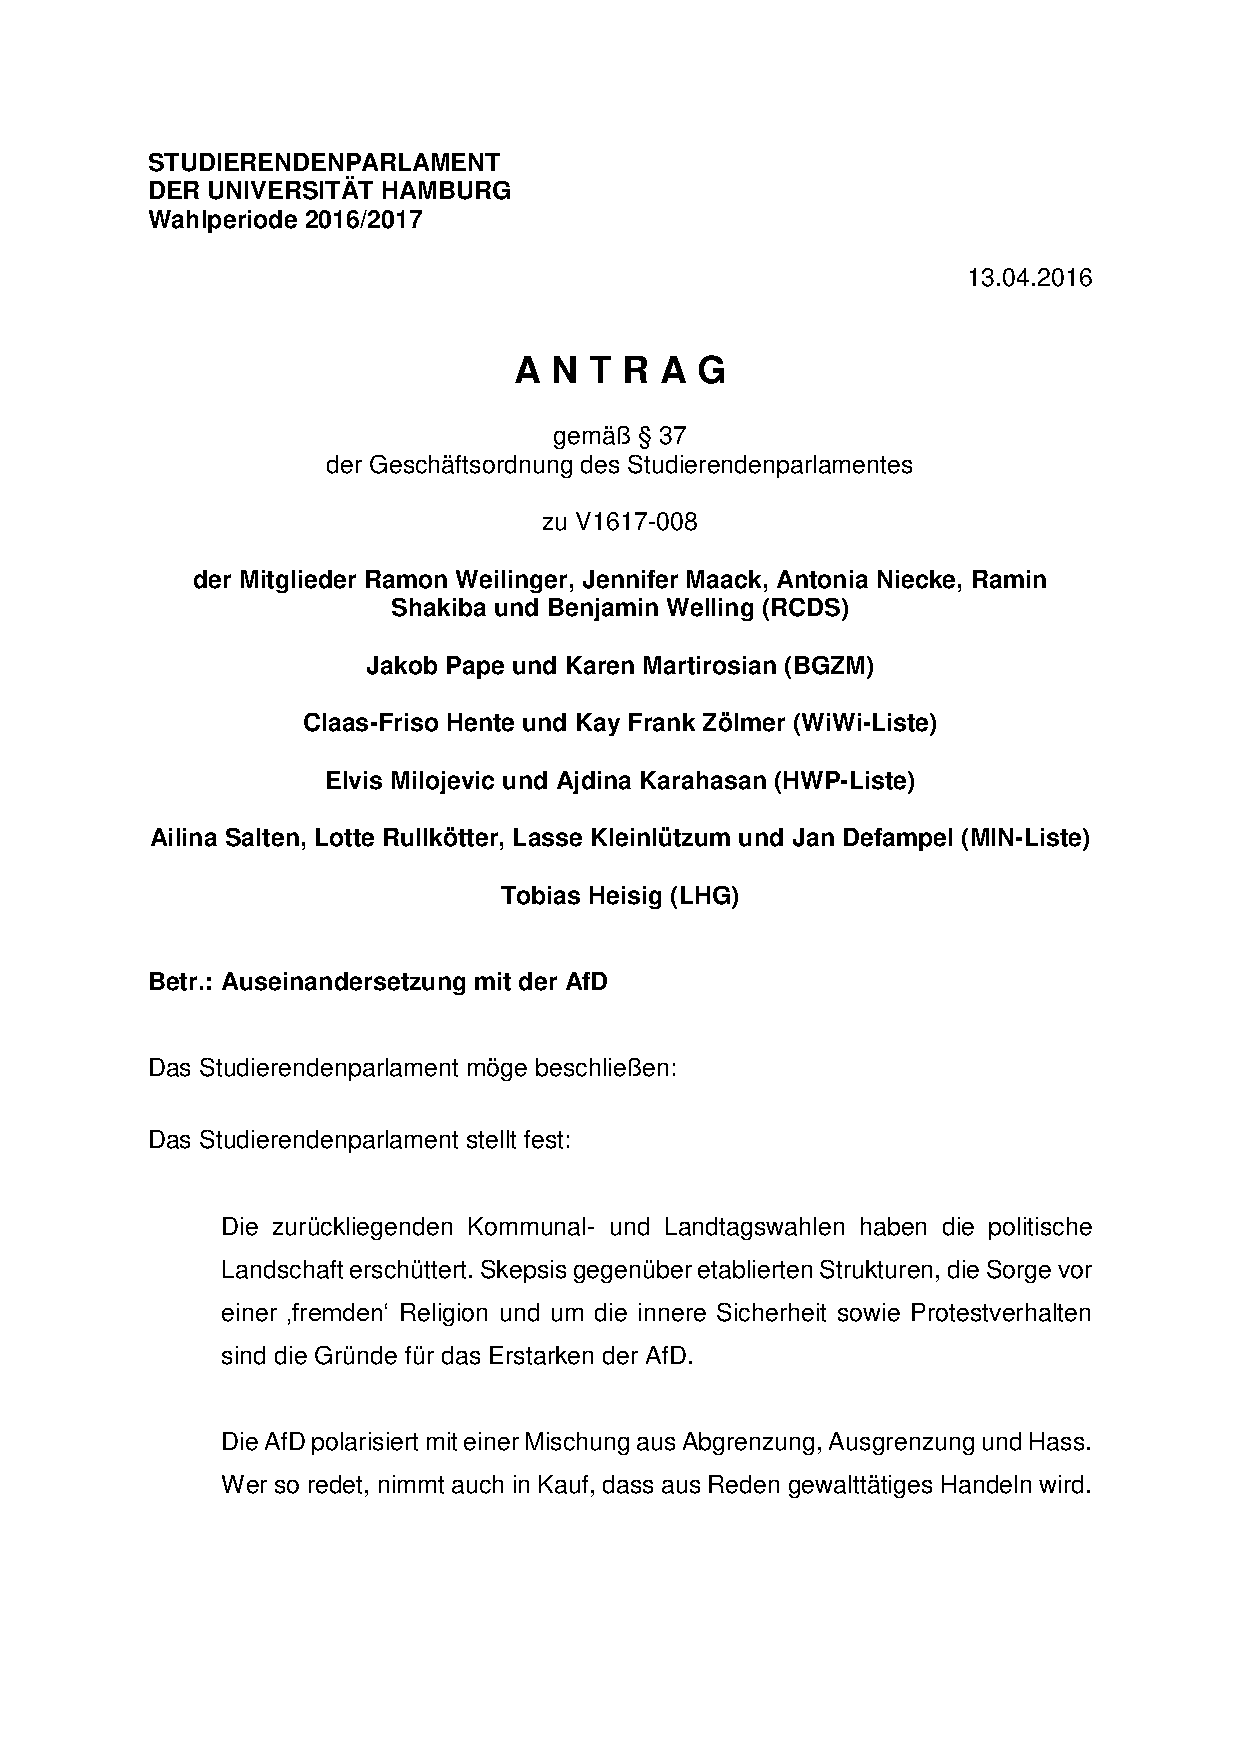
\includepdf[pages={-}]{include/ersetzungsantrag-gegen-rechts.pdf}

\end{document}
